\section{Preiskovanje}
\subsection{Neinformirani preiskovalni algoritmi}
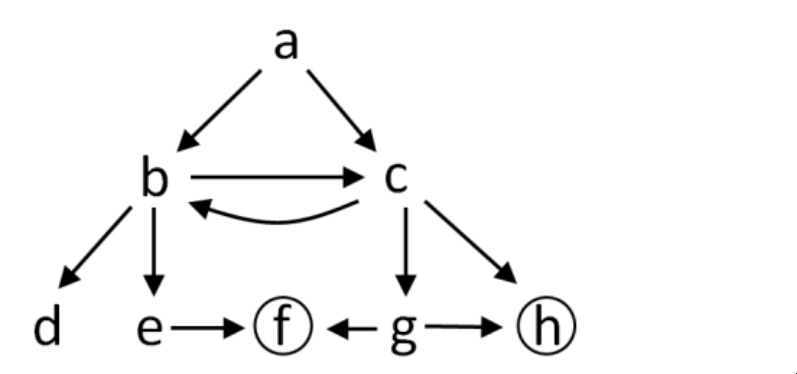
\includegraphics[width=\columnwidth]{images/neinformirano-preiskovanje.png}
\subsubsection{Iskanje v globino}
Cikle crtamo...\\
\begin{tabular}{c|c|c}
    Razvijano & Generirano & DFS list\\
    \hline
    / & a & a\\
    a & b c & b c \\
    b & c' d e & c' d e c\\
    c' & (b') g h & g h c' d e c\\
    g & f h' & f h' g h c' d e c\\
    \green{f} & koncno & koncno
\end{tabular}\\
Izboljsave (\textbf{Iskanje s sestopanjem, iterativno poglabljanje})
\subsubsection{iskanje v sirino}
\begin{tabular}{c|c|c}
Razvijano & Generirana & Vrsta\\
\hline
a & b c & [b,c]\\
b & c' d e & [c,c',d,e]\\
c & b' g h & [c',d,e,b',g,h]\\
c' & (b'') g' h' & [d,e,b',g,h,g',h']\\
d & / & [e,b',g,h,g',h']\\ 
\dots\\
h & koncno & koncno
\end{tabular}

\subsubsection{iterativno poglabljanje}
problem gobinsko omejenega iskanja -> nastavitev meje l
Mejo l postopoma povecujemo za 1, dokler ne najdemo resitve.
% itemize without spacing
\begin{itemize}[noitemsep,topsep=0pt]
    \item \textbf{popolnost}: Da
    \item \textbf{optimalnost}: Da
    \item \textbf{casovna zahtevnost} $O(b^d)$
    \item \textbf{prostorska zahtevnost} $O(bd)$
\end{itemize}
Boljse od iskanja v globino/sirino
\subsubsection{dvosmerno iskanje}
Pozenemo vzporedni iskanji od zacetka do cilja in od cilja do zacetka.\\
\textbf{Implemenatcija dvosmernega iskanja}:
\begin{itemize}[noitemsep,topsep=0pt,leftmargin=*]
    \item ciljno vozlisce mora biti znano
    \item originalni problemski prostor preslikamo v dvosmerni prosto stanj
    E1, E2 dosegljiv iz E in S1,S2,S3 dosegljiv iz S
    (S,E) -> {(S1, E1), (S1,E2), (S2, E1), (S2, E2)...}
    Vozlisce (Si, Ei) je v dvosmernem prostur ciljo vozlisce ce velja E=S (soda dolzina na isto mesto pridemo iz obeh strani) ali S->E (liha pot sosednja)
\end{itemize}
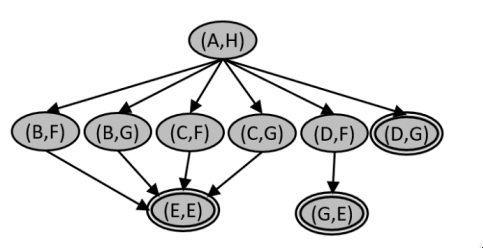
\includegraphics[width=\columnwidth]{images/dvosmerno-iskanje.png}

\subsubsection{Primerjave algoritmov}
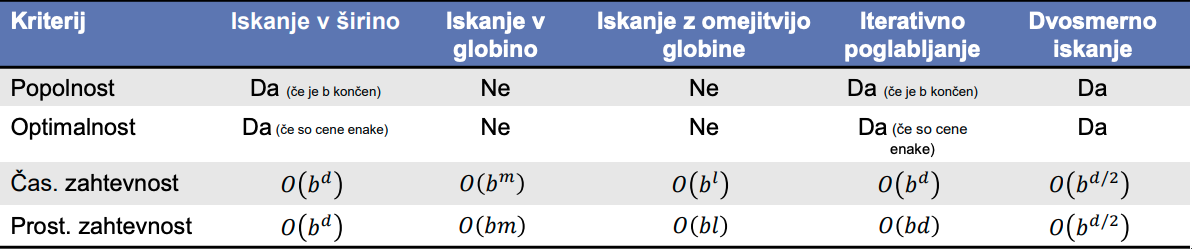
\includegraphics[width=\columnwidth]{images/neinformirano_iskanje.png}

\subsection{Informirani preiskovalni algoritmi}
Ideja: preiskovanje usmerjamo z dodatnim znanjem \textbf{hevristiko} (ocenitvena funkcija za obetavnost vozlisca)\\
- \green{optimisticna/dopustna}: $\forall n: \bm{h(n) \leq h^*(n)}$ ($h^*$ je optimalna ocena)\\
- \green{optimalna}: $h(n) = h^*(n)$\\
- \green{pesimisticna}: $h(n) \geq h^*(n)$

\subsubsection{A*}
A* is informed version of \textbf{dijkstra} (uses heuristics and pq), ce h(dopustna)=\textbf{popolna in optimalna}\\
\textbf{Casovna zahtevnost} odvisna od hevristike: $E = (h^* - h)/h^*$, $O(b^{E \cdot d})$, b-stopnja vejanja, d-globina optimalne resitve\\ 
\textbf{Prostorska zahtevnost} \textbf{problem} (hrani vsa vozlisca v spominu)\\
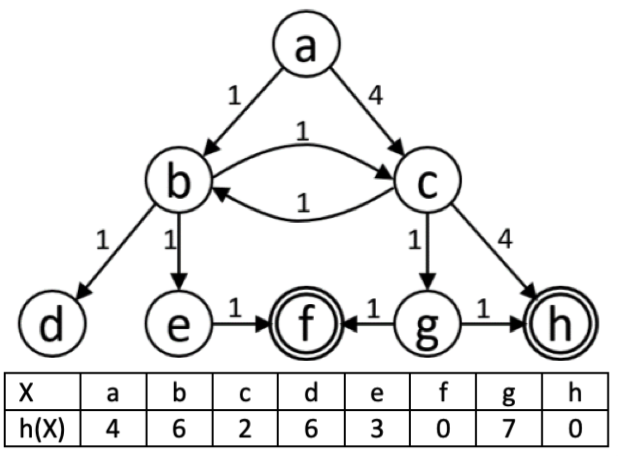
\includegraphics[width=\columnwidth]{./images/graf-a.png}\\
$f(n)=g(n)+h(n)$, g(n) cena do vozlisca, h(n) hevristika\\
Razvijamo dokler ne pridemo do ciljnega vozlisca\\
\begin{tabular}{c|c|c}
    Razvijano & Generirana & Priority Queue\\
    \hline
    / & a(4) & [] \\
    a & b(7) c(6) & $\left[ c(6), b(7)\right]$\\
    c & b'(11) g(12) h(8) & [b(7),h(8),b'(11),g(12)]\\
    b & c'(4) d(8) e(5) & [c'(4),e(5),h(8),d(8),b'(11),g(12)]\\
    \dots & \dots & \dots\\
    \magenta{f} & &
\end{tabular}

\subsubsection{IDA* (Iterative deepening A*)}
f(n) = g(n) + h(n), g(n)=cena poti do n\\
\begin{tabular}{c|c|c|c}
    Meja & Razvijano & Generirana & DFS (list)\\
    \hline
    0 & / & s(7) & /\\
    \hline
    7 & / & s(7) & s \\
      & s & a(8) b(7) c(7) & b, c\\
      & b & f(6) h(5) & f h c\\
      & f & g(7) h(9) i(11) & g h c\\
      & \underline{g} &  & 
\end{tabular}

\subsubsection{Kakovost hevristicnih funkcij}
Kakovost h ocenimo z \textbf{stevilom generiranih vozlisc} ter \textbf{efektivnim faktorjem vejanja} (N vozlisc je algoritem generiral da je na globini d nasel resitev)\\
Hocemo imeti dopustne hevristike s \textbf{cim visjimi vrednostmi} in \textbf{sprejelmjivo ceno} (casom izracuna)\\
Ce $h_2(n) \geq h_1(n), \forall n$ potem $h_2$ \textbf{dominira} $h_1$

\subsection{Nedeterministicno okolje}
Pomagajo resevati probleme z \textbf{dekompozicijo na manjse probleme}
Uporabnost:
\begin{itemize}[noitemsep,topsep=0pt,leftmargin=*]
    \item princip deli in vladaj
    \item iskanje v nedeterministicnih okoljih 
    \item igre med dvema nasprotnikoma s popolno informacijo (sah, dama)
    \item ekspertno resevanje problem
\end{itemize}

\subsubsection{AO*}
\begin{itemize}[noitemsep,topsep=0pt,leftmargin=*]
    \item posplositev A* na grafe AND/OR
    \item \textbf{popoln in optimalen} $\Leftrightarrow$ h(n) ne precenjuje dejanske cene do cilja
\end{itemize}
$F(N)$ ocena za usmerjanje preiskovanja, $H(N)$ dinamicna hevristicna ocena\\
Postopek:
\begin{enumerate}[noitemsep,topsep=0pt,leftmargin=*]
    \item Razvij najcenejse vozlisce
    \begin{itemize}[noitemsep,topsep=0pt,leftmargin=*]
        \item ce list in koncno (oznaci), preveri 3. korak, nadaljuj v 1.
        \item ce list in ni koncno (oznaci) vrednost vozlisca = $\infty$
    \end{itemize}
    \item Posodobi vse predhodnike
    \begin{itemize}[noitemsep,topsep=0pt,leftmargin=*]
        \item v AND starsih, cena starsa = $\sum$ sinov + povezava v
        \item v OR starsih, cena starsa = min(sinovi) + povezava v
    \end{itemize}
    \item Koncaj ko obstaja pot od zacetnega vozlisca, po kateri v AND vozliscih po vseh sinovih prides do cilja, v OR vozliscih v vsaj enem
\end{enumerate}
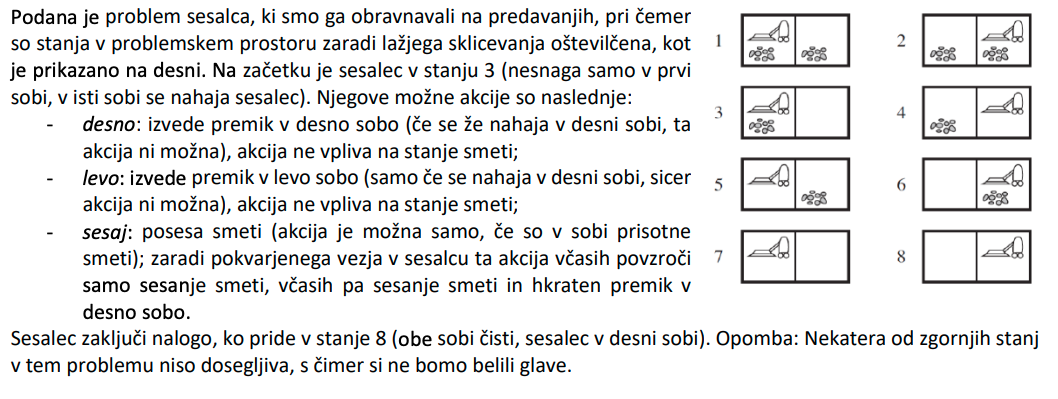
\includegraphics[width=\columnwidth]{images/nedeterminizem_ao2.png}\\
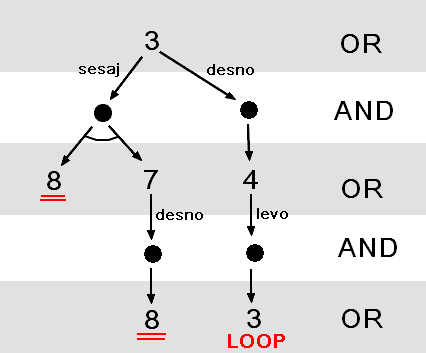
\includegraphics[width=\columnwidth]{images/nedeterminizm_ao.png}

\subsubsection{algoritem MINIMAX}
$O(n^d)$
\subsubsection{Rezanje alfa-beta}
V najbolsem primeru zmansa iz $O(b^{m \cdot d})$ na $O(b^{m \cdot d/2})$\\
V max vozliscih popravljamo \textbf{alfa}\\
V min vozliscih popravljamo \textbf{beta}\\
Iz vozlisca na otroke prenesamo par [alfa, beta]\\
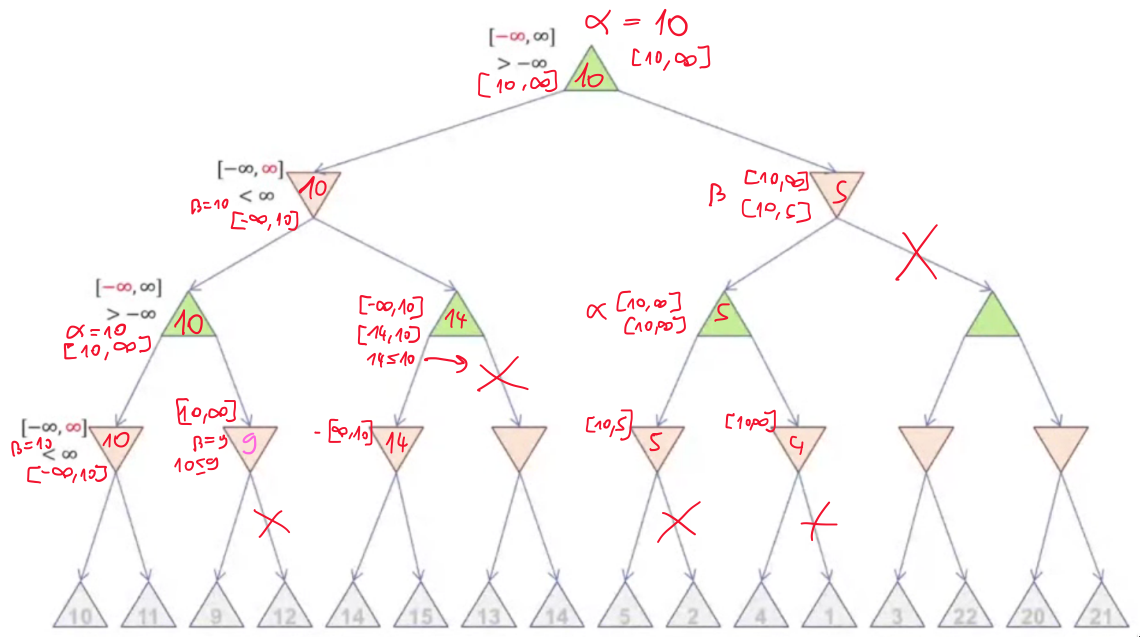
\includegraphics[width=\columnwidth]{images/alpha_beta_prunning.png}
\subsection{Lokalno preiskovalni algoritmi}
plezanje na hrib, simulirano ohlajanje, gen.algoritmi...
\subsubsection{Lokalno iskanje v snopu}
generiraj k nakljucnih zacetnih stanj\\
iz vsakegea generiraj sosede\\
izberi k najboljsih naslednikov\\
ponavljaj (iz maksimum stohasticno iskanje -> 1-verjetnost/sumvseh)
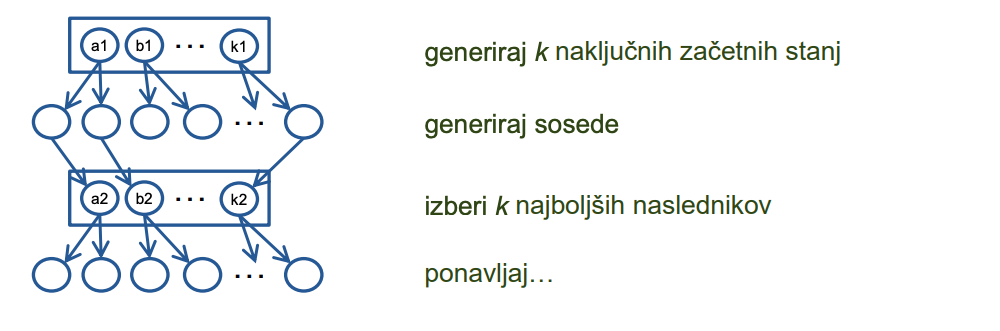
\includegraphics[width=\columnwidth]{images/lokalno_iskanje_v_snopu.png}
\blue{PRIMER:} resujemo problem iskanja izhoda iz hodnika, ki ga sestavljajo 4 sobe.
V eni izmed sob se nahaja robot, ki se lahko na vsakem koraku premakne za 1 sobo v (L) ali
v (D). Problem resujemo s preiskovanjem v snopu, ki na vsakem koraku hrani 2 aktualni stanji.\\
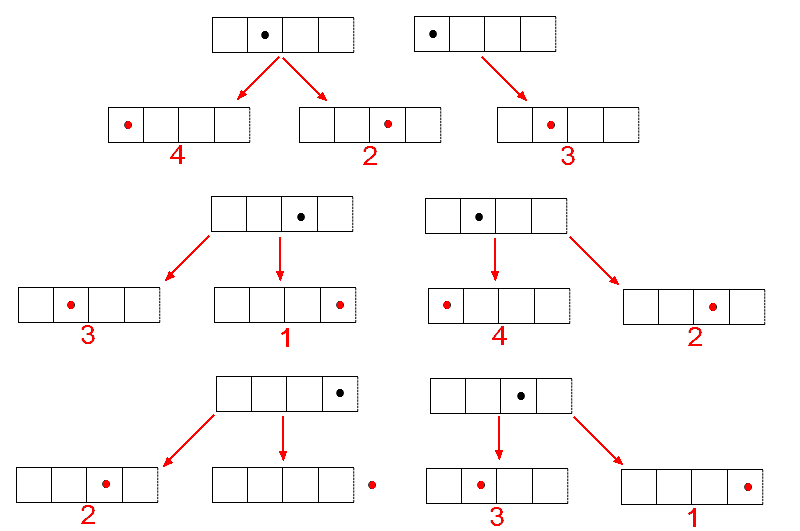
\includegraphics[width=\columnwidth]{images/iskanje_v_snopu.png}
\subsubsection{Resevanje iz lokalnih maksimumov}
\textbf{Koraki vstran}: ce ima naslendje stanje isto vrednost kriterijske funkcije, dovolimo premik
v to stanje\\
\textbf{Stohasticno} plezanje na hrib; iz mnozice boljsih stanj, verjetnstno izberemo naslednje stanje (pri 
cemer upostevamo, da imajo boljsa stanja vecjo verjetnost izbora)\\
\textbf{Nakljucni ponovni zagon}: veckrat pozeni plezanje na hrib 